\documentclass[11pt]{article}

\usepackage[a4paper,margin=1in]{geometry}
\usepackage{amsmath}
\usepackage{amssymb}
\usepackage{graphicx}
\usepackage{subcaption}
\usepackage{booktabs}
\usepackage{float}
\usepackage[colorlinks=true,linkcolor=blue,citecolor=blue,urlcolor=blue]{hyperref}

\title{MH7007 Topics in Scientific Computation I\\
\large Project Report: Algorithms, Implementation, and Analysis}
\author{Rishabh Kumar}
\date{\today}

\begin{document}
\maketitle

\begin{abstract}
This report answers Questions 1, 2, and 4 of the project sheet.  Question 1 constructs a second-order finite-difference method for a variable-coefficient elliptic boundary value problem and verifies it by a manufactured solution.  Question 2 solves a periodic linear dissipation-dispersion equation by Fourier analysis and illustrates the corresponding finite-difference Crank--Nicolson method numerically.  Question 4 studies viscous Burgers' equation, including its exact travelling wave, the conservative-form Crank--Nicolson--Leap-Frog method, and a Chebyshev collocation discretisation for the interval problem.
\end{abstract}

\section{Finite Difference Method for a Variable-Coefficient Elliptic Problem}

\subsection{Taylor expansion and the conservative flux approximation}

Let $a(x)$ be smooth and define
\begin{equation}
    P(x) = \bigl(a(x)u'(x)\bigr)'.
\end{equation}
The operator is naturally written as the derivative of a flux.  Let $h>0$ be small and introduce the half-grid points $x\pm h/2$.  By Taylor expansion,
\begin{align}
    a\left(x+\frac{h}{2}\right)u'\left(x+\frac{h}{2}\right)
    &=
    a(x)u'(x)
    +\frac{h}{2}\bigl(a u'\bigr)'(x)
    +\frac{h^2}{8}\bigl(a u'\bigr)''(x)
    +O(h^3),\\
    a\left(x-\frac{h}{2}\right)u'\left(x-\frac{h}{2}\right)
    &=
    a(x)u'(x)
    -\frac{h}{2}\bigl(a u'\bigr)'(x)
    +\frac{h^2}{8}\bigl(a u'\bigr)''(x)
    +O(h^3).
\end{align}
Subtracting and dividing by $h$ gives
\begin{equation}
    P(x)=\bigl(a u'\bigr)'(x)
    =
    \frac{
    a(x+h/2)u'(x+h/2)-a(x-h/2)u'(x-h/2)
    }{h}
    +O(h^2).
\end{equation}

Now take the uniform grid $x_j=jh$, $j=0,1,\ldots,N$, where $h=1/N$, and let
\begin{equation}
    v_j \approx u(x_j), \qquad a_{j+1/2}=a(x_j+h/2).
\end{equation}
Using centered differences for the half-grid derivatives,
\begin{equation}
    u'(x_{j+1/2}) \approx \frac{v_{j+1}-v_j}{h},
    \qquad
    u'(x_{j-1/2}) \approx \frac{v_j-v_{j-1}}{h}.
\end{equation}
Therefore
\begin{equation}
    P(x_j)
    \approx
    \frac{
    a_{j+1/2}v_{j+1}
    -(a_{j+1/2}+a_{j-1/2})v_j
    +a_{j-1/2}v_{j-1}
    }{h^2}.
    \label{eq:flux-stencil}
\end{equation}
This is second-order accurate for smooth $a$ and $u$.

\subsection{Discrete scheme for the boundary value problem}

We solve
\begin{equation}
    -\bigl(a(x)u'(x)\bigr)' + c(x)u(x)=f(x),
    \qquad 0<x<1,
    \qquad u(0)=u(1)=0,
    \label{eq:elliptic-bvp}
\end{equation}
where $a(x)\ge a_0>0$.  At the interior nodes $x_j$, $j=1,\ldots,N-1$, substituting \eqref{eq:flux-stencil} into \eqref{eq:elliptic-bvp} gives
\begin{equation}
    -\frac{a_{j-1/2}}{h^2}v_{j-1}
    +\left(\frac{a_{j+1/2}+a_{j-1/2}}{h^2}+c_j\right)v_j
    -\frac{a_{j+1/2}}{h^2}v_{j+1}
    =
    f_j,
    \label{eq:fd-scheme}
\end{equation}
where $c_j=c(x_j)$ and $f_j=f(x_j)$.  Since $v_0=v_N=0$, the unknown vector is
\begin{equation}
    V=(v_1,v_2,\ldots,v_{N-1})^T.
\end{equation}
The linear system is tridiagonal:
\begin{equation}
    A V=F,
\end{equation}
with diagonal entries
\begin{equation}
    A_{j,j}=\frac{a_{j+1/2}+a_{j-1/2}}{h^2}+c_j,
\end{equation}
upper diagonal entries
\begin{equation}
    A_{j,j+1}=-\frac{a_{j+1/2}}{h^2},
\end{equation}
and lower diagonal entries
\begin{equation}
    A_{j,j-1}=-\frac{a_{j-1/2}}{h^2}.
\end{equation}
This is the scheme implemented in the notebook using banded storage and a tridiagonal solver.

\subsection{Manufactured solution test}

For verification, choose
\begin{equation}
    u(x)=x\sin(2\pi x), \qquad
    a(x)=1+x^2, \qquad
    c(x)=e^x.
\end{equation}
This exact solution satisfies $u(0)=u(1)=0$.  We manufacture the forcing term by substituting this $u$ into the differential equation:
\begin{equation}
    f(x)=-(a(x)u'(x))' + c(x)u(x).
\end{equation}
The required derivatives are
\begin{equation}
    u'(x)=\sin(2\pi x)+2\pi x\cos(2\pi x),
\end{equation}
and
\begin{equation}
    u''(x)=4\pi\cos(2\pi x)-4\pi^2x\sin(2\pi x).
\end{equation}
Since $a'(x)=2x$,
\begin{equation}
    (a u')'=a'(x)u'(x)+a(x)u''(x),
\end{equation}
so the manufactured right-hand side is
\begin{equation}
    \begin{aligned}
    f(x)
    &=
    -2x\left(\sin(2\pi x)+2\pi x\cos(2\pi x)\right)\\
    &\quad
    -(1+x^2)\left(4\pi\cos(2\pi x)-4\pi^2x\sin(2\pi x)\right)
    +e^x x\sin(2\pi x).
    \end{aligned}
    \label{eq:manufactured-f}
\end{equation}

\begin{table}[H]
    \centering
    \caption{Maximum-norm error for the manufactured solution.  The observed rates are close to $2$, confirming the expected second-order accuracy.}
    \begin{tabular}{@{}rrrr@{}}
        \toprule
        $N$ & $h$ & $\|e_h\|_{\infty}$ & observed rate \\
        \midrule
        10  & 0.10000 & $2.911\times 10^{-2}$ & -- \\
        20  & 0.05000 & $7.113\times 10^{-3}$ & 2.033 \\
        40  & 0.02500 & $1.768\times 10^{-3}$ & 2.008 \\
        80  & 0.01250 & $4.421\times 10^{-4}$ & 2.000 \\
        160 & 0.00625 & $1.105\times 10^{-4}$ & 2.001 \\
        320 & 0.00313 & $2.762\times 10^{-5}$ & 2.000 \\
        \bottomrule
    \end{tabular}
    \label{tab:problem1-convergence}
\end{table}

\begin{figure}[H]
    \centering
    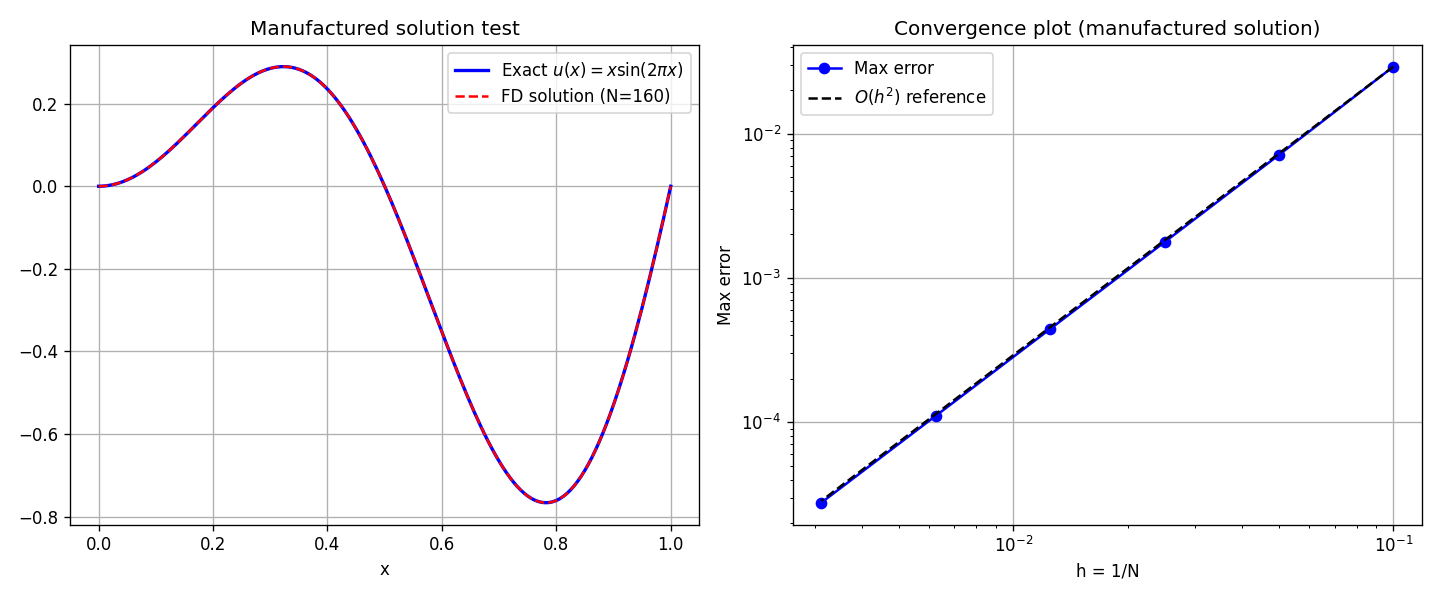
\includegraphics[width=\textwidth]{figures/manufactured_solution.png}
    \caption{Manufactured solution test.  The finite-difference solution for $N=160$ is visually indistinguishable from the exact solution, and the log-log error plot follows the \texorpdfstring{$O(h^2)$}{O(h squared)} reference line.}
    \label{fig:manufactured-solution}
\end{figure}

\subsection{Numerical solution for \texorpdfstring{$f(x)=1$}{f(x)=1}}

Finally, use the same coefficients
\begin{equation}
    a(x)=1+x^2,\qquad c(x)=e^x,
\end{equation}
but set $f(x)=1$.  The problem becomes
\begin{equation}
    -\bigl((1+x^2)u'(x)\bigr)' + e^x u(x)=1,
    \qquad 0<x<1,
    \qquad u(0)=u(1)=0.
    \label{eq:f-one-problem}
\end{equation}
The numerical computation uses $N=400$.  Since $a(x)>0$, $c(x)>0$, and $f(x)>0$, the maximum principle suggests a nonnegative interior solution.  The computed solution satisfies
\begin{equation}
    \min_j v_j \approx 0,
    \qquad
    \max_j v_j \approx 0.083874.
\end{equation}

\begin{figure}[H]
    \centering
    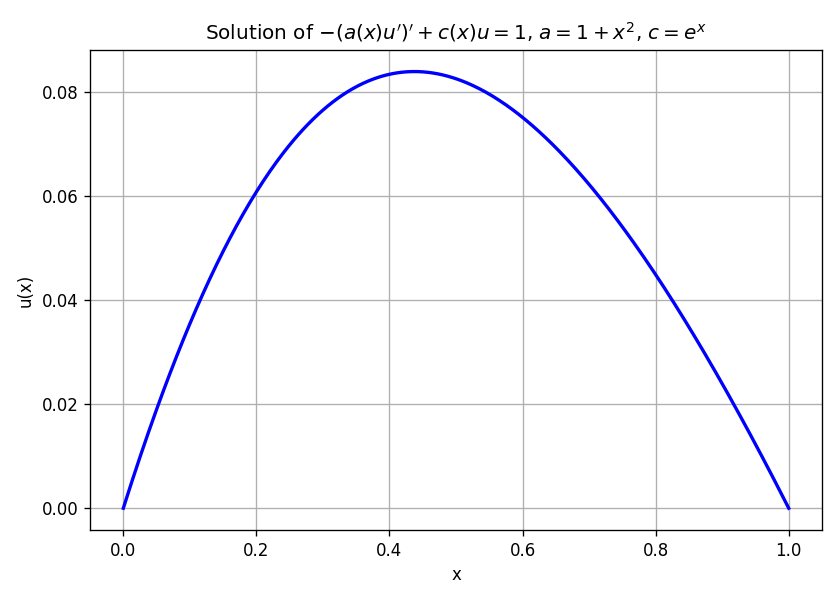
\includegraphics[width=0.72\textwidth]{figures/f_equals_1.png}
    \caption{Finite-difference solution of \eqref{eq:f-one-problem}.  The solution is nonnegative, vanishes at both boundaries, and reaches its maximum in the interior.}
    \label{fig:f-equals-one}
\end{figure}

\section{Dissipation and Dispersion}

\subsection{Fourier solution of the periodic PDE}

Consider
\begin{equation}
    u_t+a u_x=\alpha u_{xx}-\beta u_{xxx},
    \qquad -\pi<x<\pi,\quad t>0,
    \label{eq:diss-disp-pde}
\end{equation}
with $2\pi$-periodic boundary conditions and initial data
\begin{equation}
    u(x,0)=u_0(x).
\end{equation}
Assume $u_0$ is smooth and $2\pi$-periodic.  Seek a Fourier series solution
\begin{equation}
    u(x,t)=\sum_{k=-\infty}^{\infty}v_k(t)e^{ikx}.
    \label{eq:fourier-series}
\end{equation}
For one Fourier mode,
\begin{equation}
    \partial_x e^{ikx}=ik e^{ikx},\qquad
    \partial_{xx} e^{ikx}=-k^2 e^{ikx},\qquad
    \partial_{xxx} e^{ikx}=-ik^3e^{ikx}.
\end{equation}
Substituting \eqref{eq:fourier-series} into \eqref{eq:diss-disp-pde} gives the decoupled ODE
\begin{equation}
    v_k'(t)
    =
    \left(-iak-\alpha k^2+i\beta k^3\right)v_k(t).
    \label{eq:mode-ode}
\end{equation}
Thus
\begin{equation}
    v_k(t)
    =
    v_k(0)
    \exp\left\{\left(-iak-\alpha k^2+i\beta k^3\right)t\right\}.
    \label{eq:mode-solution}
\end{equation}
The full solution is therefore
\begin{equation}
    u(x,t)
    =
    \sum_{k=-\infty}^{\infty}
    v_k(0)
    \exp(-\alpha k^2 t)
    \exp\left(i\left[kx-(ak-\beta k^3)t\right]\right).
    \label{eq:fourier-solution}
\end{equation}

\subsection{Dissipation versus dispersion}

Equation \eqref{eq:fourier-solution} separates amplitude and phase effects.  The factor
\begin{equation}
    \exp(-\alpha k^2t)
\end{equation}
controls amplitude.  If $\alpha>0$, then all nonzero modes decay, and higher-frequency modes decay faster because the decay rate is proportional to $k^2$.  This is dissipation.

The oscillatory phase has angular frequency
\begin{equation}
    \omega(k)=ak-\beta k^3.
\end{equation}
The phase speed is
\begin{equation}
    c_p(k)=\frac{\omega(k)}{k}=a-\beta k^2.
\end{equation}
If $\beta\neq 0$, then different wave numbers travel at different speeds.  This frequency dependence changes the wave shape over time and is called dispersion.

\subsection{Second-order finite-difference Crank--Nicolson scheme}

On a periodic grid
\begin{equation}
    x_j=-\pi+jh,\qquad h=\frac{2\pi}{N},\qquad j=0,1,\ldots,N-1,
\end{equation}
use centered finite differences in space.  For the discrete Fourier mode $e^{ikx_j}$, the second-order symbols are
\begin{align}
    \lambda_1(k)&=\frac{i\sin(kh)}{h},\\
    \lambda_2(k)&=\frac{2(\cos(kh)-1)}{h^2},\\
    \lambda_3(k)&=\frac{i(\sin(2kh)-2\sin(kh))}{h^3}.
\end{align}
These approximate the continuous symbols $ik$, $-k^2$, and $-ik^3$ with $O(h^2)$ error.  Hence the discrete spatial symbol is
\begin{equation}
    L_k^h=-a\lambda_1(k)+\alpha\lambda_2(k)-\beta\lambda_3(k).
\end{equation}
Applying Crank--Nicolson in time to $U_k'(t)=L_k^hU_k(t)$ gives
\begin{equation}
    \frac{U_k^{n+1}-U_k^n}{\Delta t}
    =
    \frac{1}{2}L_k^h\left(U_k^{n+1}+U_k^n\right),
\end{equation}
so the Fourier-mode amplification factor is
\begin{equation}
    G_k
    =
    \frac{1+\frac{\Delta t}{2}L_k^h}
         {1-\frac{\Delta t}{2}L_k^h}.
    \label{eq:cn-factor}
\end{equation}
This is second order in time, while the centered spatial discretization is second order in space.

\subsection{Numerical illustrations}

The numerical experiments use the smooth periodic initial condition
\begin{equation}
    u_0(x)=\sin x+0.6\cos(2x)+0.3\sin(3x),
\end{equation}
with $a=1$.  Figure \ref{fig:diss-disp} compares pure advection, dissipation, and dispersion.  In the dissipative case the solution is smoothed; in the dispersive case the profile changes because the component waves propagate at different speeds.

\begin{figure}[H]
    \centering
    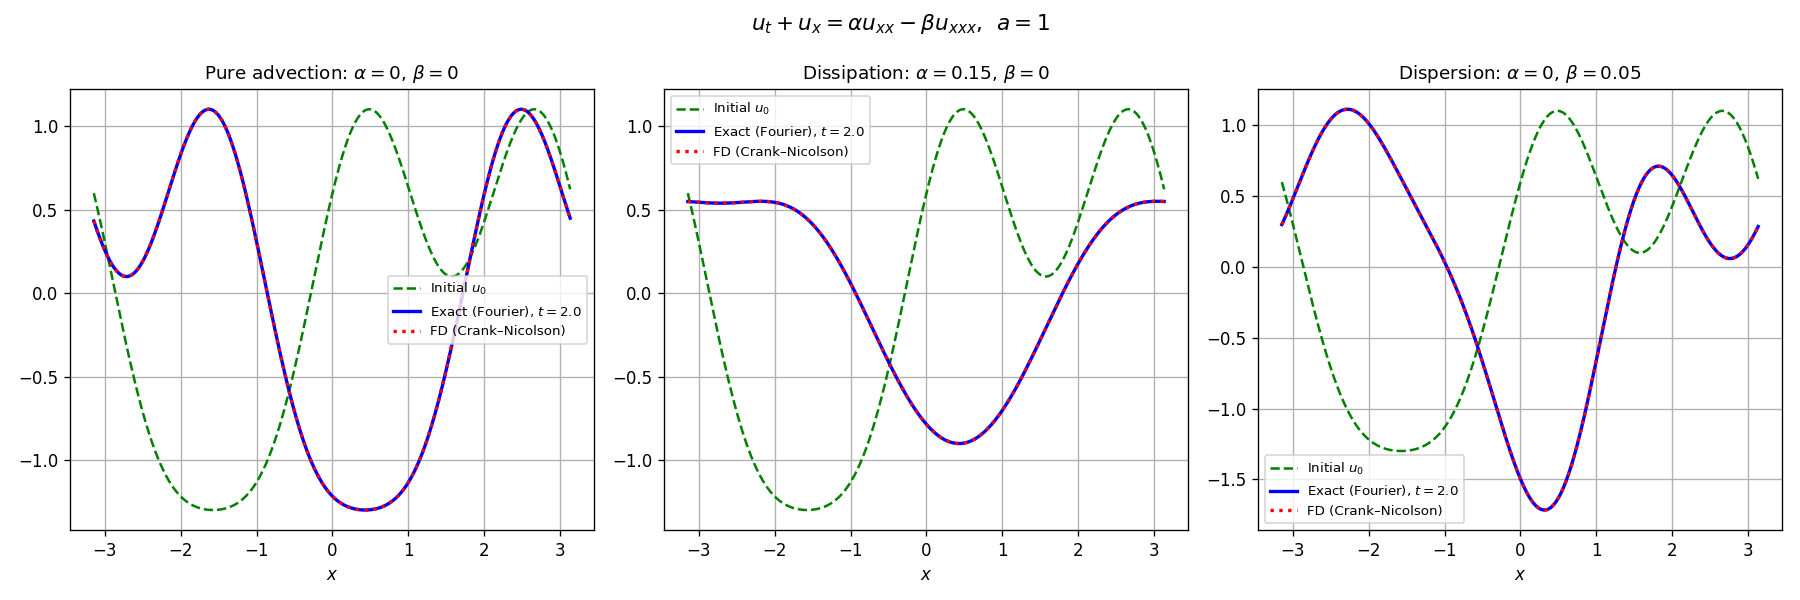
\includegraphics[width=\textwidth]{figures/dissipation_dispersion.png}
    \caption{Numerical illustration of pure advection, dissipation, and dispersion for the periodic linear equation.  The finite-difference Crank--Nicolson solution agrees closely with the exact Fourier solution.}
    \label{fig:diss-disp}
\end{figure}

\begin{table}[H]
    \centering
    \caption{Spatial convergence for the Crank--Nicolson finite-difference method with a very small time step.  The observed rates approach $2$, as expected for centered second-order spatial differences.}
    \begin{tabular}{@{}rrrr@{}}
        \toprule
        $N$ & $h=2\pi/N$ & max error & observed rate \\
        \midrule
        16  & 0.3927 & $4.765\times10^{-2}$ & -- \\
        32  & 0.1963 & $1.263\times10^{-2}$ & 1.916 \\
        64  & 0.0982 & $3.136\times10^{-3}$ & 2.009 \\
        128 & 0.0491 & $7.849\times10^{-4}$ & 1.999 \\
        256 & 0.0245 & $1.963\times10^{-4}$ & 2.000 \\
        \bottomrule
    \end{tabular}
    \label{tab:problem2-spatial}
\end{table}

\begin{table}[H]
    \centering
    \caption{Temporal convergence for Crank--Nicolson using the exact spectral spatial operator.  Removing the finite-difference spatial error exposes the clean second-order time convergence.}
    \begin{tabular}{@{}rrr@{}}
        \toprule
        $\Delta t$ & max error & observed rate \\
        \midrule
        0.10000 & $1.189\times10^{-3}$ & -- \\
        0.05000 & $2.978\times10^{-4}$ & 1.997 \\
        0.02500 & $7.447\times10^{-5}$ & 1.999 \\
        0.01250 & $1.862\times10^{-5}$ & 2.000 \\
        0.00625 & $4.655\times10^{-6}$ & 2.000 \\
        \bottomrule
    \end{tabular}
    \label{tab:problem2-temporal}
\end{table}

\begin{figure}[H]
    \centering
    \begin{subfigure}{0.49\textwidth}
        \centering
        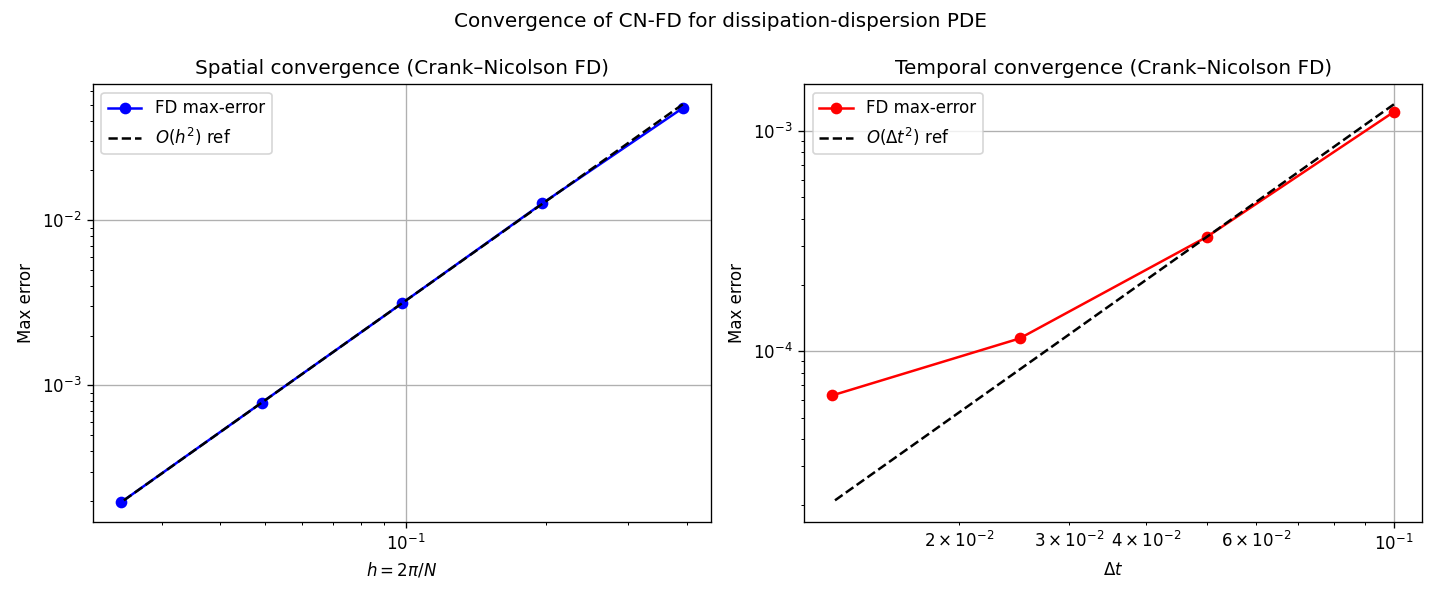
\includegraphics[width=\textwidth]{figures/convergence_fd.png}
        \caption{Finite-difference spatial and temporal convergence.}
    \end{subfigure}
    \hfill
    \begin{subfigure}{0.49\textwidth}
        \centering
        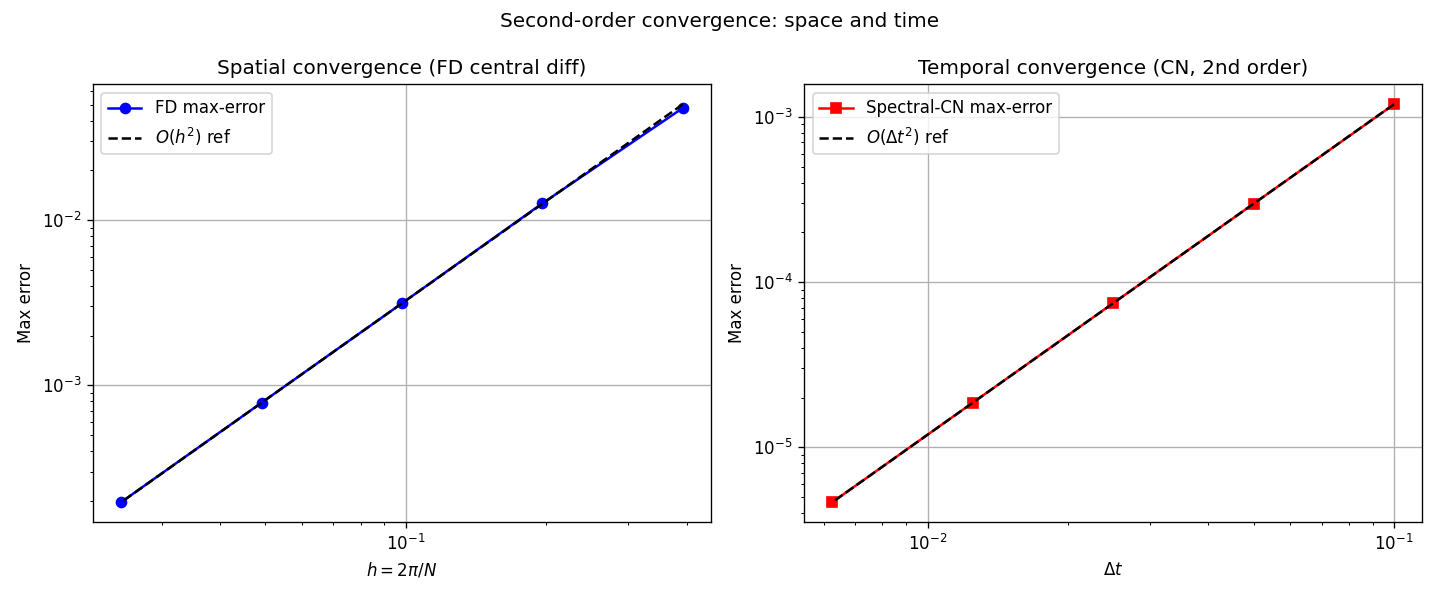
\includegraphics[width=\textwidth]{figures/convergence_spectral.png}
        \caption{Spatial convergence and spectral-in-space temporal convergence.}
    \end{subfigure}
    \caption{Convergence plots for the second-order methods.  The reference slopes confirm the expected $O(h^2)$ and $O(\Delta t^2)$ behavior.}
    \label{fig:problem2-convergence}
\end{figure}

\section{Numerical Study of the Burgers' Equation}

Consider the viscous Burgers' equation
\begin{equation}
    u_t+u u_x=\varepsilon u_{xx},
    \qquad x\in\mathbb{R},\quad t>0,
    \qquad \varepsilon>0.
    \label{eq:burgers}
\end{equation}
It is useful to write the nonlinear transport term in conservative form:
\begin{equation}
    u_t+\frac{1}{2}(u^2)_x=\varepsilon u_{xx}.
    \label{eq:burgers-conservative}
\end{equation}
This form is the natural one for the finite-difference method below, because the nonlinear term is approximated as a centred difference of the flux $u^2/2$.

\subsection{Exact travelling-wave solution}

We first show that \eqref{eq:burgers} has the exact travelling wave
\begin{equation}
    u(x,t)
    =
    \omega\left(1-\tanh\left[
    \frac{\omega}{2\varepsilon}(x-\omega t-x_0)
    \right]\right),
    \label{eq:burgers-tw}
\end{equation}
where $\omega$ and $x_0$ are constants.  Set
\begin{equation}
    y=x-\omega t-x_0,
    \qquad
    u(x,t)=w(y).
\end{equation}
Then
\begin{equation}
    u_t=-\omega w',
    \qquad
    u_x=w',
    \qquad
    u_{xx}=w''.
\end{equation}
Substitution into \eqref{eq:burgers} gives
\begin{equation}
    -\omega w'+w w'=\varepsilon w'',
\end{equation}
or, equivalently,
\begin{equation}
    -\omega w'+\left(\frac{w^2}{2}\right)'=\varepsilon w''.
\end{equation}
Integrating once with respect to $y$,
\begin{equation}
    -\omega w+\frac{w^2}{2}=\varepsilon w' + C.
\end{equation}
For the wave connecting $w(-\infty)=2\omega$ to $w(+\infty)=0$, with $w'(\pm\infty)=0$, the constant is $C=0$.  Hence
\begin{equation}
    \varepsilon w'
    =
    -\omega w+\frac{w^2}{2}
    =
    \frac{w(w-2\omega)}{2}.
    \label{eq:burgers-wave-ode}
\end{equation}
This first-order ODE is separable:
\begin{equation}
    \frac{dw}{w(w-2\omega)}
    =
    \frac{dy}{2\varepsilon}.
\end{equation}
Using partial fractions,
\begin{equation}
    \frac{1}{2\omega}
    \int\left(\frac{1}{w-2\omega}-\frac{1}{w}\right)\,dw
    =
    \frac{y}{2\varepsilon}.
\end{equation}
After absorbing the integration constant into the centre $x_0$, this gives
\begin{equation}
    w(y)=\frac{2\omega}{1+\exp(\omega y/\varepsilon)}.
\end{equation}
Using
\begin{equation}
    \frac{2}{1+e^A}=1-\tanh\left(\frac{A}{2}\right),
\end{equation}
with $A=\omega y/\varepsilon$, we obtain exactly \eqref{eq:burgers-tw}.

For a direct substitution check, set
\begin{equation}
    \eta=\frac{\omega}{2\varepsilon}(x-\omega t-x_0),
    \qquad
    u=\omega(1-\tanh\eta).
\end{equation}
Since $\eta_x=\omega/(2\varepsilon)$ and $\eta_t=-\omega^2/(2\varepsilon)$,
\begin{align}
    u_x&=-\frac{\omega^2}{2\varepsilon}\operatorname{sech}^2\eta,\\
    u_t&=\frac{\omega^3}{2\varepsilon}\operatorname{sech}^2\eta,\\
    u_{xx}&=\frac{\omega^3}{2\varepsilon^2}\operatorname{sech}^2\eta\,\tanh\eta.
\end{align}
Therefore
\begin{equation}
    u_t+u u_x
    =
    \frac{\omega^3}{2\varepsilon}
    \operatorname{sech}^2\eta\,\tanh\eta
    =
    \varepsilon u_{xx}.
\end{equation}
Thus \eqref{eq:burgers-tw} satisfies the viscous Burgers' equation.

\subsection{Crank--Nicolson--Leap-Frog scheme}

Let
\begin{equation}
    x_m=x_L+mh,
    \qquad
    t_n=nk,
    \qquad
    V_m^n\approx u(x_m,t_n).
\end{equation}
From the conservative form \eqref{eq:burgers-conservative}, approximate the time derivative at $(x_m,t_n)$ by the leap-frog difference
\begin{equation}
    u_t(x_m,t_n)
    \approx
    \frac{V_m^{n+1}-V_m^{n-1}}{2k}.
\end{equation}
The nonlinear flux is treated explicitly at time level $n$:
\begin{equation}
    \frac{1}{2}(u^2)_x(x_m,t_n)
    \approx
    \frac{1}{2}
    \frac{(V_{m+1}^n)^2-(V_{m-1}^n)^2}{2h}
    =
    \frac{(V_{m+1}^n)^2-(V_{m-1}^n)^2}{4h}.
\end{equation}
The diffusion term is averaged by Crank--Nicolson over the two leap-frog levels:
\begin{equation}
    u_{xx}(x_m,t_n)
    \approx
    \frac{1}{2h^2}
    \left(
    \delta_x^2 V_m^{n+1}
    +
    \delta_x^2 V_m^{n-1}
    \right),
\end{equation}
where
\begin{equation}
    \delta_x^2 V_m^n
    =
    V_{m+1}^n-2V_m^n+V_{m-1}^n.
\end{equation}
The CNLF scheme is therefore
\begin{equation}
    \frac{V_m^{n+1}-V_m^{n-1}}{2k}
    +
    \frac{(V_{m+1}^n)^2-(V_{m-1}^n)^2}{4h}
    =
    \frac{\varepsilon}{2h^2}
    \left(
    \delta_x^2 V_m^{n+1}
    +
    \delta_x^2 V_m^{n-1}
    \right).
    \label{eq:cnlf-raw}
\end{equation}
Multiplying by $2k$ and setting
\begin{equation}
    \mu=\frac{\varepsilon k}{h^2},
\end{equation}
we obtain the linear tridiagonal solve at each time step:
\begin{equation}
    V_m^{n+1}-\mu\delta_x^2V_m^{n+1}
    =
    V_m^{n-1}+\mu\delta_x^2V_m^{n-1}
    -
    \frac{k}{2h}
    \left((V_{m+1}^n)^2-(V_{m-1}^n)^2\right).
    \label{eq:cnlf-solve}
\end{equation}
The nonlinear term is explicit, while the viscous part is implicit.  Consequently each update requires only a tridiagonal linear solve.  Since the method is two-step, the computation needs $V^0$ and $V^1$.  In the travelling-wave convergence tests, $V^1$ is taken from the exact solution to isolate the CNLF discretisation error.

\subsection{Local truncation error}

Let $u_m^n=u(x_m,t_n)$ be the exact smooth solution sampled on the grid and let $q=u^2$.  The centred time difference satisfies
\begin{equation}
    \frac{u_m^{n+1}-u_m^{n-1}}{2k}
    =
    u_t+\frac{k^2}{6}u_{ttt}+O(k^4).
\end{equation}
For the nonlinear conservative flux,
\begin{equation}
    \frac{(u_{m+1}^n)^2-(u_{m-1}^n)^2}{4h}
    =
    \frac{1}{2}\frac{q(x_m+h,t_n)-q(x_m-h,t_n)}{2h}
    =
    \frac{1}{2}q_x+\frac{h^2}{12}q_{xxx}+O(h^4).
\end{equation}
For the Crank--Nicolson diffusion average,
\begin{equation}
    \frac{1}{2h^2}
    \left(
    \delta_x^2 u_m^{n+1}
    +
    \delta_x^2 u_m^{n-1}
    \right)
    =
    u_{xx}
    +
    \frac{k^2}{2}u_{xxtt}
    +
    \frac{h^2}{12}u_{xxxx}
    +
    O(k^4+k^2h^2+h^4).
\end{equation}
Substituting the exact solution into the discrete scheme and using \eqref{eq:burgers-conservative}, the local truncation error has leading terms
\begin{equation}
\begin{aligned}
    \tau_m^n
    &=
    \frac{k^2}{6}u_{ttt}
    +\frac{h^2}{12}(u^2)_{xxx}
    -\varepsilon
    \left(
    \frac{k^2}{2}u_{xxtt}
    +
    \frac{h^2}{12}u_{xxxx}
    \right)
    +O(k^4+k^2h^2+h^4).
\end{aligned}
\end{equation}
Therefore
\begin{equation}
    \tau_m^n=O(k^2+h^2).
\end{equation}
With a second-order startup and stability on the smooth branch of the solution, the expected global error is also second order in space and time.

\subsection{Travelling-wave numerical test and convergence}

For the verification experiment, use
\begin{equation}
    \omega=0.5,\qquad
    \varepsilon=0.1,\qquad
    x_0=3,\qquad
    -5\le x\le 5,\qquad
    T=2.
\end{equation}
With $h=k=10^{-3}$, the notebook computation gives
\begin{equation}
    \|e(T)\|_{\infty}=4.548\times 10^{-7}.
\end{equation}

\begin{figure}[H]
    \centering
    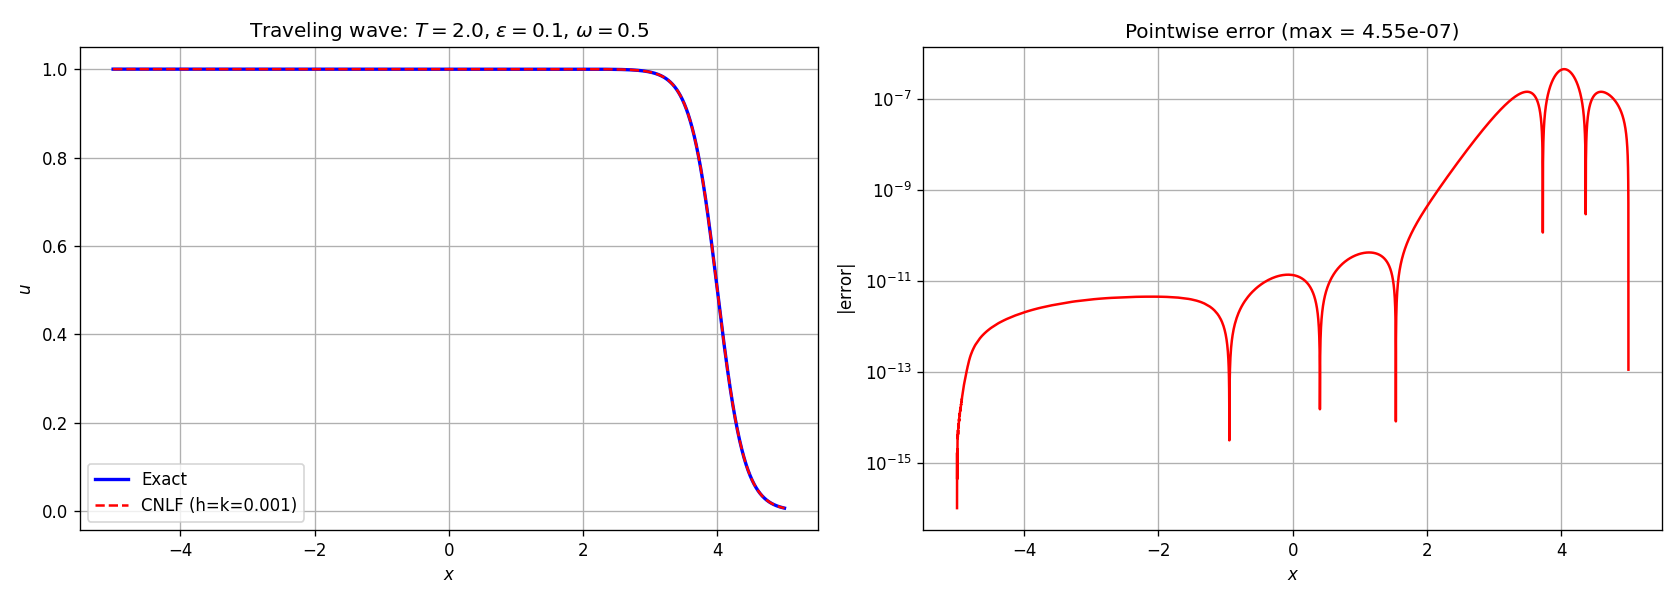
\includegraphics[width=\textwidth]{figures/traveling_wave.png}
    \caption{CNLF approximation of the exact Burgers travelling wave at $T=2$, together with the pointwise absolute error.}
    \label{fig:burgers-traveling-wave}
\end{figure}

\begin{table}[H]
    \centering
    \caption{Coupled refinement study for the travelling-wave solution.  The slope is essentially second order when $h=k$.}
    \begin{tabular}{@{}rrr@{}}
        \toprule
        $h=k$ & $\|e(T)\|_{\infty}$ & observed rate \\
        \midrule
        0.0400 & $6.056\times10^{-4}$ & -- \\
        0.0200 & $1.513\times10^{-4}$ & 2.001 \\
        0.0100 & $3.790\times10^{-5}$ & 1.997 \\
        0.0050 & $9.485\times10^{-6}$ & 1.998 \\
        \bottomrule
    \end{tabular}
    \label{tab:burgers-coupled}
\end{table}

\begin{table}[H]
    \centering
    \caption{Separate temporal convergence with $h=2.5\times10^{-4}$.}
    \begin{tabular}{@{}rrrr@{}}
        \toprule
        $k$ & $\|e\|_{\infty}$ & $\|e\|_2$ & $L^2$ rate \\
        \midrule
        $8.0\times10^{-3}$ & $1.906\times10^{-5}$ & $3.663\times10^{-6}$ & -- \\
        $4.0\times10^{-3}$ & $4.742\times10^{-6}$ & $9.125\times10^{-7}$ & 2.005 \\
        $2.0\times10^{-3}$ & $1.165\times10^{-6}$ & $2.250\times10^{-7}$ & 2.020 \\
        $1.0\times10^{-3}$ & $2.708\times10^{-7}$ & $5.316\times10^{-8}$ & 2.081 \\
        \bottomrule
    \end{tabular}
    \label{tab:burgers-time}
\end{table}

\begin{table}[H]
    \centering
    \caption{Separate spatial convergence with $k=10^{-4}$.}
    \begin{tabular}{@{}rrrr@{}}
        \toprule
        $h$ & $\|e\|_{\infty}$ & $\|e\|_2$ & $L^2$ rate \\
        \midrule
        $4.0\times10^{-2}$ & $8.461\times10^{-4}$ & $1.584\times10^{-4}$ & -- \\
        $2.0\times10^{-2}$ & $2.117\times10^{-4}$ & $3.963\times10^{-5}$ & 1.999 \\
        $1.0\times10^{-2}$ & $5.295\times10^{-5}$ & $9.911\times10^{-6}$ & 1.999 \\
        $5.0\times10^{-3}$ & $1.324\times10^{-5}$ & $2.478\times10^{-6}$ & 2.000 \\
        \bottomrule
    \end{tabular}
    \label{tab:burgers-space}
\end{table}

\begin{figure}[H]
    \centering
    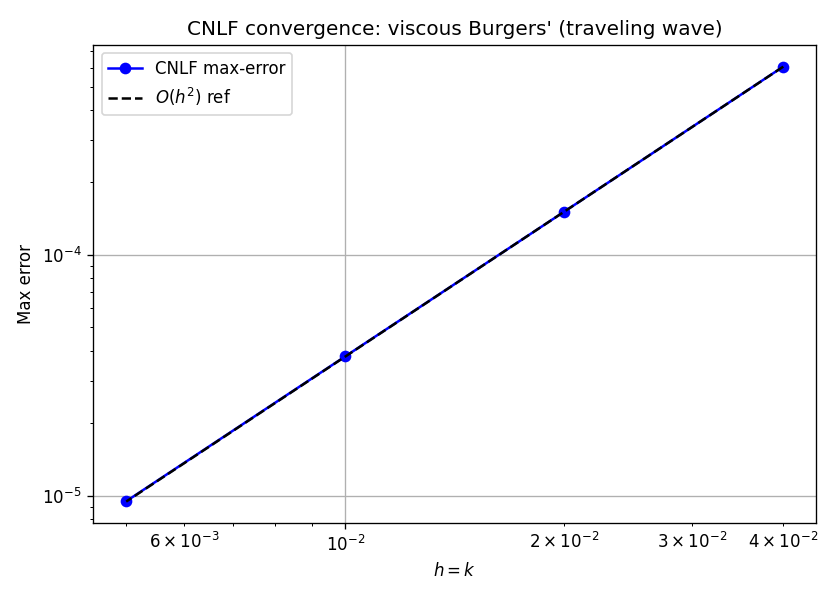
\includegraphics[width=0.72\textwidth]{figures/burgers_convergence.png}
    \caption{Coupled second-order convergence for the CNLF method on the travelling-wave problem.}
    \label{fig:burgers-convergence}
\end{figure}

\subsection{Chebyshev collocation for the interval problem}

The last part considers Burgers' equation on $(-1,1)$ with
\begin{equation}
    u(\pm1,t)=0,
    \qquad
    u(x,0)=-\sin(\pi x),
    \qquad
    \varepsilon=0.02,
    \qquad
    T=0.995.
    \label{eq:burgers-interval}
\end{equation}
Fourier collocation is the standard spectral collocation method for periodic domains, because trigonometric basis functions automatically respect periodicity.  On a bounded nonperiodic interval, the analogous standard spectral collocation method uses Chebyshev polynomials and Chebyshev--Lobatto points.  These nodes cluster near the endpoints, which is useful for viscous Burgers' equation when steep gradients develop near boundaries.

For polynomial degree $N$, define
\begin{equation}
    x_j=\cos\left(\frac{j\pi}{N}\right),
    \qquad
    j=0,1,\ldots,N.
\end{equation}
Let $U_j(t)\approx u(x_j,t)$.  If $p_N$ is the interpolating polynomial through the nodal values, then differentiation at the nodes is represented by a dense matrix $D$:
\begin{equation}
    p_N'(x_i)\approx \sum_{j=0}^{N}D_{ij}U_j.
\end{equation}
For $i\neq j$,
\begin{equation}
    D_{ij}
    =
    \frac{c_i}{c_j}
    \frac{(-1)^{i+j}}{x_i-x_j},
    \qquad
    c_0=c_N=2,\quad c_j=1\quad(1\le j\le N-1),
\end{equation}
and the diagonal is chosen so each row sums to zero:
\begin{equation}
    D_{ii}=-\sum_{j\neq i}D_{ij}.
\end{equation}
The second derivative is represented by
\begin{equation}
    D^{(2)}=D^2.
\end{equation}

Using the conservative form, the semi-discrete collocation system is
\begin{equation}
    \dot U+\frac{1}{2}D(U\odot U)=\varepsilon D^2U,
    \label{eq:cheb-semidiscrete}
\end{equation}
where $\odot$ denotes componentwise multiplication.  Imposing $U_0=U_N=0$ and writing $I$ for the interior indices, the CNLF update becomes
\begin{equation}
    \left(I-\varepsilon k D^2_{II}\right)U_I^{n+1}
    =
    U_I^{n-1}
    +
    \varepsilon k (D^2U^{n-1})_I
    -
    \frac{k}{2}\left(D\bigl((U^n)^2\bigr)\right)_I.
    \label{eq:cheb-cnlf}
\end{equation}
As before, the method is two-step.  The notebook uses one nonlinear Crank--Nicolson startup step:
\begin{equation}
    U^1-U^0
    +
    \frac{k}{4}D\left((U^1)^2+(U^0)^2\right)
    -
    \frac{\varepsilon k}{2}D^2(U^1+U^0)
    =
    0,
    \label{eq:cheb-startup}
\end{equation}
restricted to interior nodes and solved by Newton's method.

For the computation, the notebook uses
\begin{equation}
    N=96,\qquad
    k=10^{-3},\qquad
    \varepsilon=0.02,\qquad
    T=0.995.
\end{equation}
Figure \ref{fig:cheb-collocation} shows the resulting Chebyshev-collocation CNLF solution and selected profiles.

\begin{figure}[H]
    \centering
    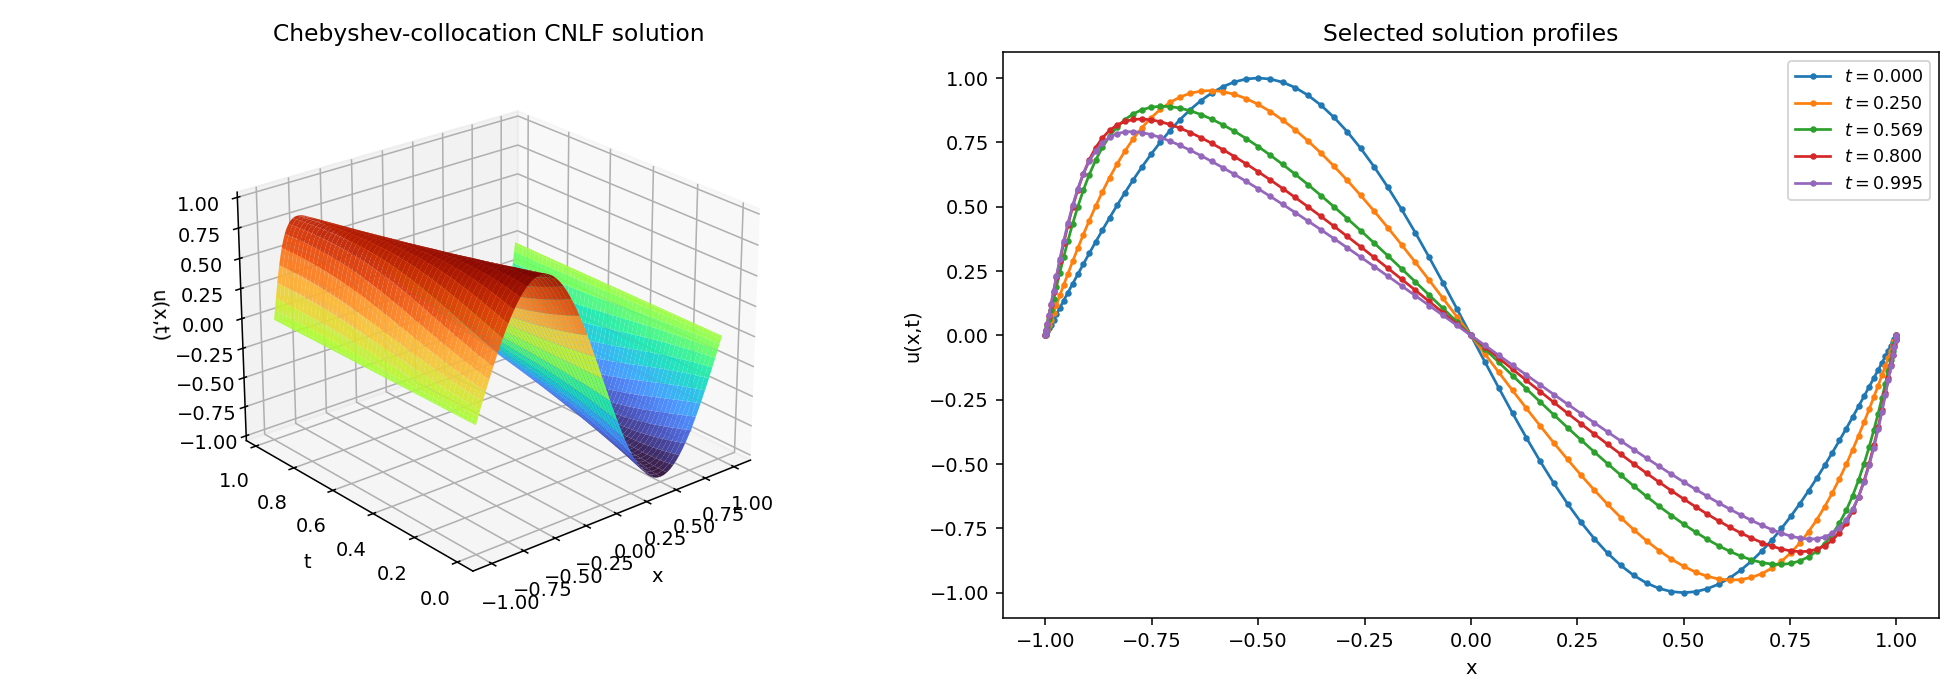
\includegraphics[width=\textwidth]{figures/chebyshev_collocation.png}
    \caption{Chebyshev-collocation CNLF solution of Burgers' equation on $(-1,1)$ with $u(\pm1,t)=0$ and $u(x,0)=-\sin(\pi x)$.}
    \label{fig:cheb-collocation}
\end{figure}

\begin{figure}[H]
    \centering
    
\includegraphics[width=0.72\textwidth]{figures/burgers_sine.png}
    \caption{Finite-difference CNLF reference profiles for the same interval problem.  The Chebyshev collocation method captures the same steepening and smoothing behaviour using a spectral spatial discretisation.}
    \label{fig:burgers-sine}
\end{figure}

\section{Conclusion}

For Question 1, the conservative half-grid flux discretization gives a tridiagonal second-order finite-difference method for the variable-coefficient elliptic problem.  The manufactured solution test confirms the $O(h^2)$ convergence rate, and the $f(x)=1$ computation produces a physically consistent nonnegative solution.

For Question 2, Fourier analysis shows precisely how the parameter $\alpha$ produces dissipation through amplitude decay and how $\beta$ produces dispersion through frequency-dependent phase speed.  The periodic Crank--Nicolson finite-difference method reproduces these effects and demonstrates second-order accuracy in space and time.

For Question 4, the viscous Burgers' equation admits an exact tanh travelling wave, obtained either by travelling-wave reduction or by direct substitution.  The CNLF method follows cleanly from the conservative form of Burgers' equation by combining leap-frog time differencing, explicit centred flux differencing, and Crank--Nicolson averaging of the viscous term.  Taylor expansion gives local truncation error $O(k^2+h^2)$, and the numerical tests confirm second-order behaviour.  On the nonperiodic interval $(-1,1)$, Chebyshev collocation provides the corresponding spectral spatial discretisation and resolves the steep solution profiles with endpoint-clustered nodes.

\end{document}
